\section{Analysis}
This chapter describes the first step of this project, the research of published technical reports and tools which are considered interesting for this project.
\subsection{BloodHound / SharpHound}
%Lukas
BloodHound describes himself on his wiki page on GitHub as followed:
\begin{quotation} \ \\
\textit{''BloodHound is a single page Javascript web application, built on top of Linkurious, compiled with Electron, with a Neo4j database fed by a PowerShell/C\# ingestor. \\
BloodHound uses graph theory to reveal the hidden and often unintended relationships within an Active Directory environment. Attacks can use BloodHound to easily identify highly complex attack paths that would otherwise be impossible to quickly identify. Defenders can use BloodHound to identify and eliminate those same attack paths. Both blue and red teams can use BloodHound to easily gain a deeper understanding of privilege relationships in an Active Directory environment.''} 
%\cite{}
\end{quotation}
\ \\
BloodHound was tested in the test environment describes later in this chapter. Both, the C\# and Python ingestors were successfully installed and tested. The only problem which occurred was that the Python-ingestor does not yet run on the latest Python release. One must have a Python 2.7.x version installed to run the scripts successfully.
The most interesting part about BloodHound is the way they retrieve their data.

\subsection{LogonTracer}
%Claudio

\subsection{WEFFLES}
%Lukas

\subsection{Microsoft Security Complience Toolkit}
%Claudio

\subsection{Microsoft Monitoring Active Directory for Signs of Compromise}
%Claudio und ein paar Worte zum Anhang

\subsection{MITRE ATT\&CK}
%Claudio

\subsection{JPCert - Detecting Lateral Movement through Tracking Event Logs}
%Lukas

\subsection{JPCert - Detecting Lateral Movement in APTs}
%Lukas

\subsection{Test environment}
A virtual network was set up on Azure-Cloud as a test environment. The test network was set up in the cloud so that the development team can access the network regardless of its location. The test network consists of a Windows server and two Windows clients. Active Directory service was configured on the server to manage the client computer. The following operating systems were installed in this test network: \\
\\
\textbf{Server:}
\begin{itemize}
    \item Windows Server 2016
\end{itemize}
\textbf{Clients:}
\begin{itemize}
    \item Windows 10 Pro, Version 1709
\end{itemize}
The network is structured as followed:\\
\begin{figure}[H]
    \centering
    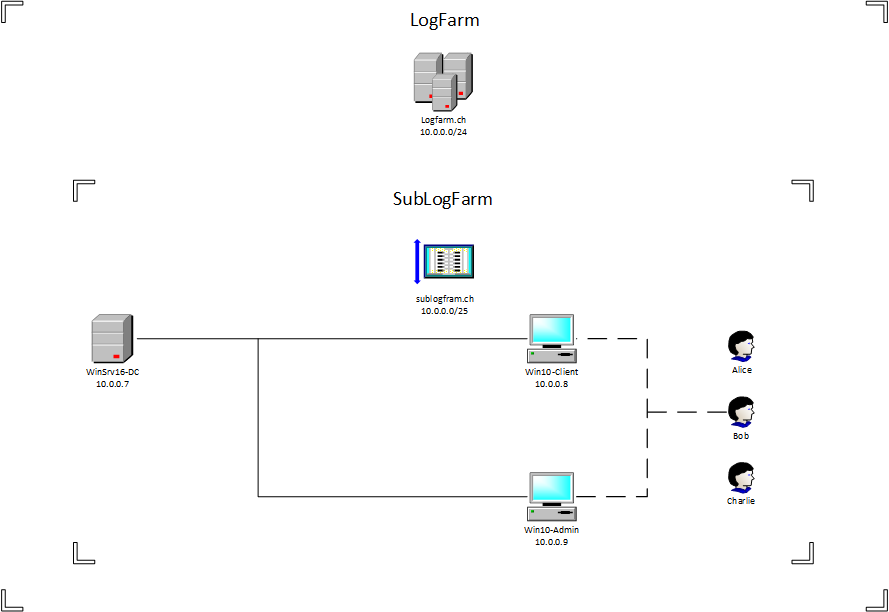
\includegraphics[width=0.9\linewidth]{assets/testnetwork.png}
    \caption{test environment}
\end{figure}
\subsubsection{Users}
Three different users were configured:
\begin{table}[H]
    \centering
    \begin{tabular}{p{4cm} p{8cm}} \hline
        \textbf{Name} & \textbf{Permissions}  \\ \hline
        alice & administration  \\ \hline
        bob & user  \\ \hline
        charlie & user  \\ \hline
    \end{tabular}
    \caption{Angaben Lukas Kellenberger}
\end{table}